\subsection{Câu lệnh if - else}
Ở câu lệnh if, chương trình chỉ thực thi khối lệnh nếu điều kiện vào là đúng. Trong nhiều trường hợp, ta cũng cần phải xử lý chương trình khi điều kiện vào là sai. Việc sử dụng từ khoá \texttt{else} sẽ giải quyết được trường hợp trên.\par
Cấu trúc của câu lệnh if - else:\par
\texttt{if <condition>:}\par
\qquad \texttt{//if block's code}\par
\texttt{else:}\par
\qquad \texttt{//else block's code}\par
\begin{figure}[h]
	\centering
	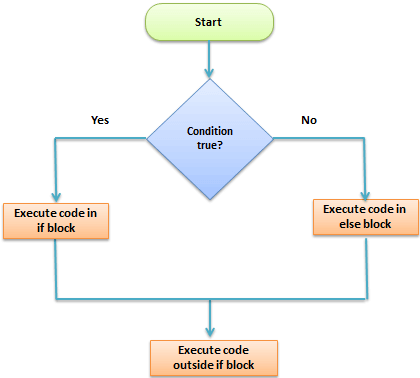
\includegraphics{img/if_else}
	\caption{Mô tả cách thức hoạt động của câu lệnh if - else}
\end{figure}
\newpage
\textbf{Ví dụ:} Chương trình nhập vào một số nguyên, kiểm tra đó là số chẵn hay lẻ:\\
\rule{\linewidth}{0.2mm}\par
\begin{linenumbers}
	\texttt{number = \textcolor{red}{int}(\textcolor{blue}{input}("Type a number: "))}\par
	\texttt{\textcolor{red}{if} number \% 2 == 0:}\par
	\qquad \texttt{\textcolor{blue}{print}("\%d is an even number." \% number)}\par
	\texttt{\textcolor{red}{else}:}\par
	\qquad \texttt{\textcolor{blue}{print}("\%d is an odd number." \% number)}\par
\end{linenumbers}
\rule{\linewidth}{0.2mm}\par
\noindent
\resetlinenumber
Kết quả cho ra ở Console:\\
\rule{\linewidth}{0.2mm}\par
\begin{linenumbers}
	\texttt{Type a number: 11}\par
	\texttt{11 is an odd number.}
\end{linenumbers}
\rule{\linewidth}{0.2mm}\par
\resetlinenumber
\newpage
\textbf{Ví dụ:} Chương trình xếp loại, với điểm >= 8 xếp loại giỏi, >= 7 xếp loại khá và còn lại là trung bình:\\
\rule{\linewidth}{0.2mm}\par
\begin{linenumbers}
	\texttt{score = \textcolor{red}{float}(\textcolor{blue}{input}("Type your score: "))}\par
	\texttt{\textcolor{red}{if} score >= 8:}\par
	\qquad \texttt{\textcolor{blue}{print}("Excellent")}\par
	\texttt{\textcolor{red}{else}:}\par
	\qquad \texttt{\textcolor{red}{if} score >= 7:}\par
	\qquad \qquad \texttt{\textcolor{blue}{print}("Good")}\par
	\qquad \texttt{\textcolor{red}{else}:}\par
	\qquad \qquad \texttt{\textcolor{blue}{print}("Medium")}\par
\end{linenumbers}
\rule{\linewidth}{0.2mm}\par
\noindent
\resetlinenumber
Kết quả cho ra ở Console:\\
\rule{\linewidth}{0.2mm}\par
\begin{linenumbers}
	\texttt{Type your score: 6.2}\par
	\texttt{Medium}
\end{linenumbers}
\rule{\linewidth}{0.2mm}\par
\resetlinenumber
\newpage